\documentclass{article}
\usepackage{graphicx} % Required for inserting images
\usepackage{subcaption}
\def\changemargin#1#2{\list{}{\rightmargin#2\leftmargin#1}\item[]}
\let\endchangemargin=\endlist 
\usepackage{amsmath}
\usepackage{multicol,multirow}



\title{Mathematical Foundations of Image Synthesis}
\author{Utshav Saha (2305077)}
\date{July 2026}

\begin{document}

\maketitle

\section{Introduction}
Image synthesis is the process of generating images from mathematical and algo-rithmic descriptions. Modern graphics systems rely on \textbf{precise mathematical models} and efficient computation. \emph{Even small numerical errors} can result in visible artifacts in rendered images. Typical formulations involve scalar values such as $x$, indexed parameters
like $I_{ij}$, and exponential terms $e^{x^2}$. These elements are combined to simulate realistic lighting behavior.

\section{Core Components}
\subsection{Rendering Pipeline}
The rendering pipeline consists of the following stages:

\begin{itemize}
    \item Scene Definition
    \item Camera Configuration
    \item[-] Light Placement
\end{itemize}

\begin{changemargin}{-1cm}{0cm} 
\textbf{Important} Shading Model\end{changemargin}
\begin{itemize}
    \item[-] Diffuse Shading
    \item[-] Specular Highlights
\end{itemize}

\subsection{Execution Order}
\begin{enumerate}
    \item Input Processing
    \item Ray Construction
        \begin{enumerate}
            \item Primary Rays
            \item Secondary Rays
        \end{enumerate}
    \item Intersection Evaluation
        \begin{itemize}
            \item Object Hit Test
        \end{itemize}
\end{enumerate}

\section{Mathemetical Modeling}
Light interaction with surfaces can be expressed using the following equations.

\begin{equation}
    L = I_{ij} \cdot \cos(\theta) + R
\end{equation}

$$k = \frac{ab}{cd}$$

\begin{align*}
    f(x) &= x^2 + 2x + 1\\
        &= (x+1)^2\tag{2}
\end{align*}

\[
\lvert y \rvert = 
\begin{cases}
    y & \text{if } x \geq 0 \\
    -y  & \text{if } x < 0
\end{cases}
\]

\[
p(t) = 
\begin{cases}
    0 & \text{if } t < 0 \\
    e^-t  & \text{if } 0 \leq t < 3 \\
    ln(t-2) & \text{if } t \geq 3
\end{cases}
\]

$$ \mathcal{N}(x_i, \mu, \sigma) = \frac{1}{\sqrt{2\pi}\sigma}e^{-{\frac{ ({x_i-\mu})^2}{2\sigma^2}}} $$

\section{Performance Comparison}

\begin{table}[!h]
    \centering
    \begin{tabular}{|c|c|c|}
    \hline
         Method & Accuracy & Time Complexity  \\ \hline
         Rasterization & Medium & $O(n)$ \\ \hline 
        \multirow{2}{2cm}{Ray Tracing} & High & $O(n^2)$ \\
        & Very High & $O(n^3)$ \\ \hline
        \multicolumn{2}{|c|}{Hybrid Method} & $O(n^2)$ \\ \hline
    \end{tabular}
    \caption{Comparison of Image Synthesis Techniques}
    \label{tab:comparison}
\end{table}

The results in Table \ref{tab:comparison} highlight the trade-off between accuracy and computational cost.

\clearpage

\section{Visual Illustration}
\begin{figure}[ht]
    \centering
    \begin{subfigure}[b]{0.3\linewidth}
        \centering
        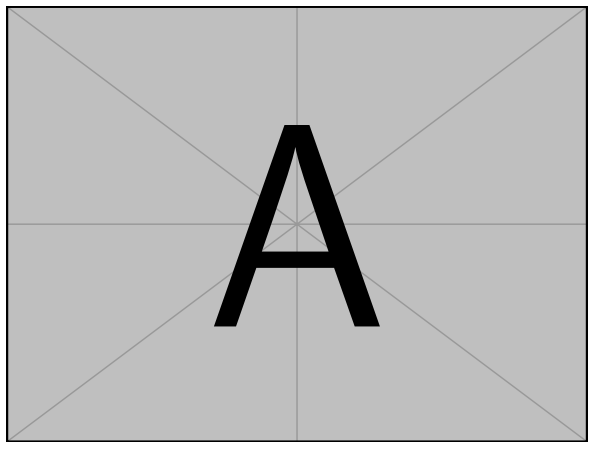
\includegraphics[width=1\linewidth]{A (1).PNG}
        \caption{Output A}
        \label{fig:placeholder}
    \end{subfigure}
    \hfill
    \begin{subfigure}[b]{0.3\linewidth}
        \centering
        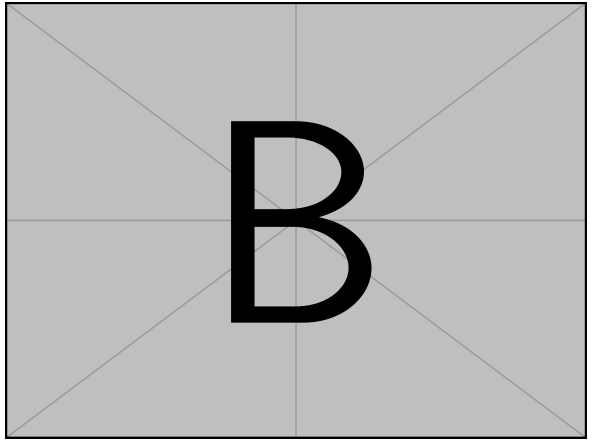
\includegraphics[width=1\linewidth]{B (1).PNG}
        \caption{Output B}
        \label{fig:placeholder}
    \end{subfigure}
    \hfill
    \begin{subfigure}[b]{0.3\linewidth}
        \centering
        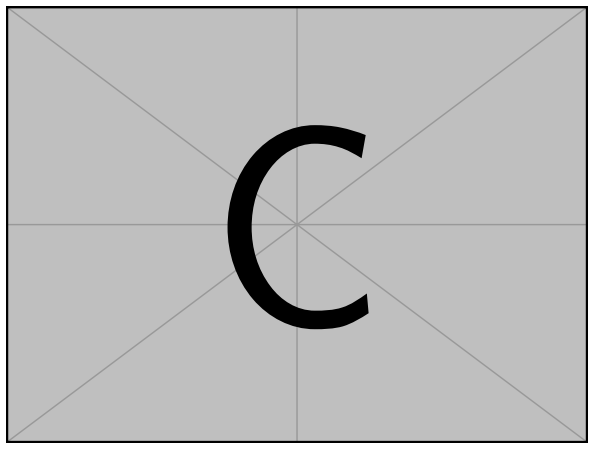
\includegraphics[width=1\linewidth]{C (1).PNG}
        \caption{Output C}
        \label{fig:placeholder}
    \end{subfigure}
    
    \caption{Comparison of three rendering outputs.}
    \label{fig:outputs}
\end{figure}

Figure \ref{fig:outputs} compares three different rendering outputs arranged in a single row.

\section{Conclusion}
Image synthesis combines \underline{mathematical precision}, algorithmic design, and efficient implementation. As scene complexity increases, choosing the appropriate method becomes critical for balancing quality and performance.

\end{document}
